
%(BEGIN_QUESTION)
% Copyright 2007, Tony R. Kuphaldt, released under the Creative Commons Attribution License (v 1.0)
% This means you may do almost anything with this work of mine, so long as you give me proper credit

Choose the appropriate switch terminals to land wires connecting the two pressure switches to the PLC in order to satisfy the requirements of the ``online'' program display (showing color highlighting), assuming pressure A is 14 PSI and pressure B is 70 PSI:

$$\includegraphics[width=15.5cm]{i02882x01.eps}$$

\underbar{file i02882}
%(END_QUESTION)





%(BEGIN_ANSWER)

Color in the online program display reveals a path for ``virtual power'' in the ladder-logic ``circuit''.  This means every colored ``contact'' is in its closed state, while every uncolored ``contact'' is in its open state.  Since we see that only the normally-open ``contact'' instructions are colored while all the normally-closed ``contact'' instructions are uncolored, we know that all bit states must be one (1).
 
\vskip 10pt

A ``one'' (1) input bit state is caused by real electrical power applied to that PLC input channel.  This means both inputs must be energized by pressure switches that are {\it closed}.

\vskip 10pt

Since pressure switch A is experiencing a pressure of only 14 PSI (below the trip threshold of 25 PSI), it must be in its resting state.  Thus, we must wire its {\it normally-closed (NC)} contact to channel {\tt I:0/3} of the PLC.

\vskip 10pt

Since pressure switch B is experiencing a pressure of 70 PSI (above the trip threshold of 55 PSI), it must be in its actuated state.  Thus, we must wire its {\it normally-open (NO)} contact to channel {\tt I:0/1} of the PLC.

$$\includegraphics[width=15.5cm]{i02882x02.eps}$$

%(END_ANSWER)





%(BEGIN_NOTES)


%INDEX% PLC, relating I/O status to virtual elements
%INDEX% PLC, wiring: properly connecting input devices to a PLC

%(END_NOTES)


